\documentclass{article}
\usepackage{algorithmicx}
\usepackage{algpseudocode}
\usepackage{graphicx}

\begin{document}
{\noindent \Huge Problema a resolver:}
\newline \newline  El problema esta dado por la siguiente situaci\'on: nos encontramos en un extremo de un puente (afuera de \'el) y queremos llegar al otro extremo, bajo ciertas circunstancias y, si es posible hacer esto, hacerlo de la "mejor manera" (mas adelante se detallar\'a qu\'e significa esto y por qu\'e podr\'ia no ser posible atravesar el puente). El puente est\'a hecho con una cantidad \textit{n} de tablones seguidos y, algunos de ellos pueden estar rotos. Cuando esto suceda, vamos a querer saltar estos tablones rotos al atravesar el puente, pisando siempre tablones sanos cuando estemos avanzando.\newline
Tenemos una cantidad fija tablones seguidos que podemos saltar, la denominaremos \textit{c}, as\'i podemos ver que, si el puente tiene, en alg\'un momento, una cantidad \textit{$k > c$} de tablones rotos \textbf{seguidos}, entonces claramente no tendremos manera de atravesarlo ya que, intuitivamente, podemos pensar que, en el mejor de los casos (donde mejor significa estar lo m\'as alejados posibles del comienzo del puente) podr\'iamos estar en el tablon sano anterior (anterior inmediato) al primero de esos \textit{k} tablones rotos y, a\'un as\'i no podr\'iamos atravesar el puente ya que no podemos saltar m\'as de \textit{c} tablones seguidos, por lo tanto en cualquier otro caso (donde nos encontr\'aramos en un tabl\'on anterior al anterior inmediato del primero de los \textit{k} rotos por ejemplo), estar\'iamos en una situaci\'on similar porque eventualmente llegar\'iamos al tabl\'on sano que es el anterior inmediato al primero de los \textit{k} y quedar\'iamos estancados de la misma manera.
\newline En el caso en el que no se de la situaci\'on descripta anteriormente (es decir, en el caso en el cual s\'i podamos atravesar el puente), vamos a querer dar la menor cantidad de saltos (la "mejor manera").
\newline \newline Presentamos algunos ejemplos graficos junto a sus soluciones y las secuencias que lo representan. Los circulos con el A y el B determinan el punto de partida y el punto de llegada, ambos fuera del puente. Los tablones rotos est\'an pintados de negro.

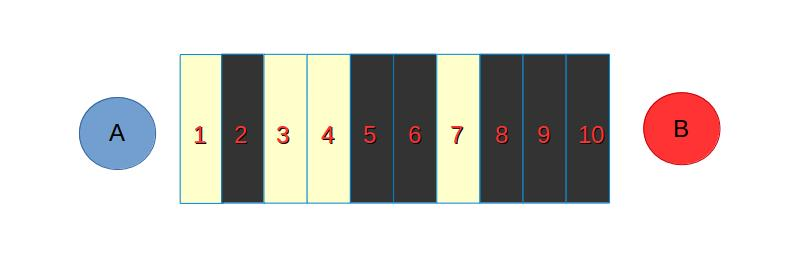
\includegraphics[width=\textwidth,height=\textheight,keepaspectratio
]{ejemplopuente1.jpg}
\begin {flushleft}
En este ejemplo, \textit{$n = 10$} y el puente se escribe como 10 c 0 1 0 0 1 1 0 1 1 1.
\newline Si \textit{$c = 3$}, entonces la soluci\'on est\'a dada por caer en los tablones 4 7 11. Notar que en realidad no existe un trabl\'on numerado con el 11, pero cuando exista una soluci\'on, para indicar que llegamos al punto de llegada, diremos que saltamos a un tabl\'on mayor estricto que la cantidad de tablones del puente (o sea, que estamos efectivamente fuera del puente).
Si tuvieramos el mismo puente pero con \textit{$n = 2$}, claramente no existir\'ia una soluci\'on ya que, si bien podr\'iamos llegar al tabl\'on 7 sin problemas, una vez ah\'i no tendr\'iamos manera de saltar el 8, 9 y 10 que est\'an rotos.\end {flushleft}
\vspace{1cm}
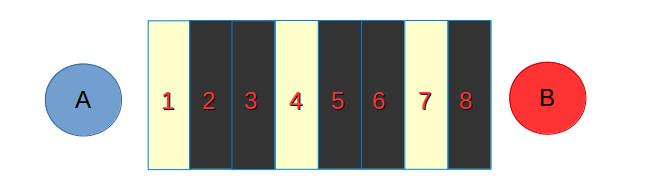
\includegraphics[width=\textwidth,height=\textheight,keepaspectratio
]{ejemplopuente2.jpg}
\begin {flushleft}Este otro puente se representa como 8 c 0 1 1 0 1 1 0 1.
\newline Si \textit{$c = 2$} entonces la soluci\'on es 1 4 7 9.
\newline Si \textit{$c = 1$} entonces no habr\'ia soluci\'on ya que hay 2 tablones rotos seguidos (esto ocurre dos veces en este caso particular pero con que ocurra una ya no hay soluci\'on posible).
\newline Si \textit{$c = 3$} la soluci\'on es  4 7 9.
\end {flushleft}

\vspace{1cm}
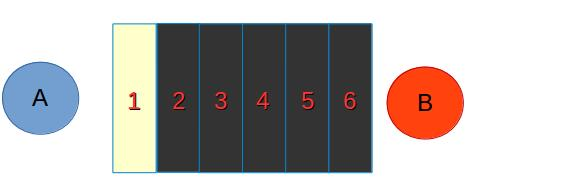
\includegraphics[width=\textwidth,height=\textheight,keepaspectratio
]{ejemplopuentes3.jpg}
\begin {flushleft}
Finalmente introducimos este ultimo ejemplo del puente 6 c 0 1 1 1 1 1.
Siguiendo la misma l\'ogica que ven\'iamos teniendo, podemos ver que este puente no tiene soluci\'on para \textit{$c < 5$}. Si \textit{$c = 5$} entonces la soluci\'on es 1 7 y s\'i \textit{$c > 5$} la soluci\'on es 7.
\end{flushleft}
\newpage
{\noindent \Huge Resoluci\'on:}
\newline \newline
La idea basicamente es ir recorriendo el puente (tabl\'on por tabl\'on) e ir almacenanando cual es el \'ultimo tabl\'on sano (lo llamaremos \textit{ultimosano}) desde el comienzo del puente hasta el tabl\'on de la iteraci\'on actual \textit{i} (notar que \textit{ultimosano} podr\'ia ser \textit{i}), los tablones que conformar\'ian la soluci\'on en el caso de que exista y la cantidad de tablones por los que pasamos desde el \'ultimo tabl\'on que agregu\'e a la soluci\'on (sin contarlo) hasta el tabl\'on de la iteraci\'on actual (cont\'andolo), llamaremos a esta \'ultima variable \textit{saltados}.
\newline Eventualmente podemos llegar a una iteraci\'on donde \textit{$saltados = c + 1$} (\textit{c} es dato y representa la cantidad de tablones como m\'aximo que puedo saltar) y, si no llegamos a esta iteraci\'on quiere decir que terminamos de recorrer todos los tablones del puente antes de llegar a pasar por \textit{$c + 1$} tablones desde el \'ultimo sano.
\newline Analicemos el primer caso donde efectivamente llegamos a esa iteraci\'on donde vale \textit{$saltados = c + 1$}: si llegamos a este punto significa que estamos parados en el tabl\'on mas lejano al cual puedo llegar saltando desde el \'ultimo tabl\'on que agregu\'e a la soluci\'on (porque si puedo saltar \textit{c} tablones seguidos desde donde estoy, entonces caigo en el tabl\'on \textit{$c + 1$}). Entonces nuevamente pueden pasar dos cosas: 1) \textit{$i - ultimosano > c$} (que la cantidad de tablones entre el tabl\'on de la iteraci\'on actual \textit{i} hasta \textit{ultimosano} sea mas grande que c) 2) \textit{$i - ultimosano <= c$}. Si estamos en 1) voy a tener una cantidad mayor estricta que \textit{c} de tablones seguidos donde ninguno de ellos es un tabl\'on sano (la \'ultima vez que asign\'e un valor a \textit{ultimosano} fue o bien antes de empezar a iterar, o sea cuando estoy fuera del puente, o en un tabl\'on que dista a m\'as de \textit{c} tablones del actual), esto quiere decir que est\'an todos rotos y, como no puedo saltar una cantidad mayor que \textit{c} de tablones seguidos, concluimos que no existe una soluci\'on al problema. Ahora bien si estamos en 2), entonces quiere decir que existe un tabl\'on sano (y est\'a almacenado en \textit{ultimosano} entre el \'ultimo que agregu\'e a la soluci\'on  (si no agregu\'e ninguno, entonces este tabl\'on representa el punto de partida fuera del puente) y el tabl\'on representado por la iteraci\'on actual \textit{i} y este tabl\'on NO es el \'ultimo que agregu\'e a la soluci\'on (de ser as\'i no estar\'iamos en este caso). Entonces lo que hacemos es agregar \textit{ultimosano} a la soluci\'on y actualizar el valor de \textit{saltados} para que represente la cantidad de tablones que salt\'e desde el \'ultimo que agregu\'e a la soluci\'on (que es el que agregamos reci\'en, \textit{ultimosano}) hasta llegar al tabl\'on de la iteraci\'on actual \textit{i}. Una vez hecho esto, repetimos el proceso descripto con la siguiente iteraci\'on.
\newline
Dado que los tablones que deben ser soluci\'on se agregan a la misma cuando nos encontramos en una iteraci\'on \textit{i} en la cual vale \textit{$saltados = c + 1$}, podr\'ia suceder que terminemos de iterar y no hayamos pasado por esta iteraci\'on \textit{i}. Esto quiere decir que a partir del \'ultimo tabl\'on que agregu\'e a la soluci\'on, hay una cantidad menor estricta que \textit{$c + 1$} tablones y por lo tanto, puedo saltarlos todos, alcanzando as\'i el punto de llegada fuera del puente.
\newline Cuando terminamos de iterar todos los tablones del puente, agregamos como el \'ultimo "tabl\'on" de la soluci\'on, un n\'umero mayor estricto que \textit{n} para indicar que estamos fuera del puente. 

A continuaci\'on, presentamos el pseudoc\'odigo que hace lo que describimos arriba:
\vspace{0.4cm}
\begin{algorithmic}[1]
\Procedure{ResolverPuente}{$puente,c$}
	\State $ultimosano\gets -1$
	\State $saltados\gets 0$
	\State $solucion\gets \emptyset$
	\State $n\gets cantidadTablones(puente)$
	\For{$i\gets 1, n$}
		\State $saltados++$
		\If{$puente[i]\gets 0$}
			\State $ultimosano\gets i$
		\EndIf
		\If{$saltados == c + 1$}
			\If{$i - ultimosano > c \vee ultimosano == - 1$}
				\State no hay soluci\'on, termino
			\EndIf
			\State $agregar(soluci$\'o$n, i)$
			\State $saltados = i - ultimosalto$
		\EndIf
	\EndFor
	\State $agregar(soluci$\'o$n, size(puente) + 1)$
\EndProcedure
\end{algorithmic}


\end{document}